\chapter{Implementation}
\label{implementation}
This code base is intended to be treated as a tool box for the optimization of acoustic networks.  While a fully-functional application is provided, its intent is to serve as a template for integrating various functionalities.  It is expected that researchers will want to define and use customized versions of the provided functions (herein referred to as ''subfunctions'').  To support this, the framework utilizes generic ''dispatcher functions'' and dictionary-based parameter passing.  

\subsection{Parameter Dictionary}
\label{parameterDictionary}
The framework takes as an input to the main program a dictionary of named values (\texttt{params}), and passes it throughout the program.  This allows for dispatcher functions with concrete function signatures (volatile parameters can be incorporated into the parameter dictionary), and sub-functions with widely varied signatures.  The benefit of this is that the function signatures of the dispatcher functions will rarely need to be changed, leading to a stable but flexible framework. The cost of this approach is that data validation of dictionary-based parameters must be preformed before the execution of sub-functions in order to avoid run-time errors within the varied sub-functions.  


\subsection{Sub-Functions}
\label{sub-functions}
Section \ref{design} discusses the framework's conceptual models such as Goodness computation and animal modeling.  These models have loose operational requirements that can be thought of as roles.  For example, it is expected that an animal model populates the Behavior Grid, and that an Evaluation Algorithm populate the Goodness Grid.  As long as a user-customized sub-function fulfills its role within the prescribed model (suppressing a given location, populating a Grid, etc.), it can be easily integrated into the framework.

\subsection{Dispatcher Functions}
\label{dispatcherFunctions}
The primary purpose of dispatcher functions is to create a uniform interface within the framework for calling various sub-functions.  Each model has a corresponding dispatcher function, and these dispatcher functions are responsible for preparing and calling sub-functions which belong to that model.  For example, the Animal Model dispatcher is responsible for functions which populate the Behavior Grid.  A dispatcher function performs a series of if-else checks over one or more ''option'' variables in the parameter dictionary, and executes the corresponding sub-function.  Once a user defines a new sub-function, they should add the new sub-function as an option within the corresponding dispatcher.  This will allow a user to use the new sub-function by calling the dispatcher function with the new option.  Any sub-function-specific data validation should be done at the beginning of the program, before any computationally-expensive operations are preformed, by the \texttt{checkParams()} function (Section~\ref{checkParams}).


\subsection{Major Modules}
\label{majorModules}
\subsubsection{Parameter Checking}
\label{checkParams}
As previously mentioned in Section~\ref{parameterDictionary}, the cost of flexible inputs is substantial data validation.  Within the framework, data validation should occur early on so that errors can be identified before too much time has been invested in computation or data-loading.  To this end, the \texttt{checkParams()} function is provided to handle all data validation and reporting.  The function takes in the \texttt{params} parameter dictionary and a \texttt{stop} boolean (set to True by default).  The function and validates all internal dependencies, reporting any errors found, and halting the program if \texttt{stop} is True.  The function also assigns necessary default values if no user-defined values are provided.  The function returns the validated \texttt{params} parameter dictionary (with default values if necessary).  

\subsubsection{File Output}
The File Output Module is responsible for generating graphical and textual results for the framework.  The primary function in this module is the \texttt{graph()} function, which takes in three parameters, a \texttt{result} parameter dictionary, a \texttt{params} parameter dictionary, and a boolean, \texttt{showPlots}.  The \texttt{result} parameter dictionary, contains results (Table~\ref{resultDict}) from successfully completing a simulation.  The \texttt{params} parameter dictionary contains parameters passed into the program, and generated by the framework.  \texttt{showPlots} directs file output.  If \texttt{showPlots} is set to False, the function writes the output files described in Section~\ref{outputFiles} to disk, and returns a dictionary of file paths that point to the the newly written files.  If \texttt{showPlots} is set to False, then the same results are displayed within an R session instead of being written to disk.  Filenames for output files follow a \texttt{timestamp-FileName} convention, where \texttt{timestamp} is a user-specified string (defaulting to the time the request passed Parameter Validation) and \texttt{FileName} is a contextual identifier (''GoodnessGrid'', ''BehaviorGrid'', etc).  Graphic output from this module is generated using the R \texttt{graphics} package.  Zip file creation uses the 
R \texttt{zip} package.

\begin{table}[ht]
	\begin{tabular}{l l l}
		Key	&	Value &	Description\\
		\hline
		\texttt{topographyGrid}	&	The Bathymetry Grid			&	An alias for the unmodified Bathymetry Grid.\\
		\texttt{behaviorGrid}	&	The Behavior Grid			&	The unmodified Behavior Grid.\\
		\texttt{goodnessGrid}	&	The Goodness Grid			&	The unmodified Goodness Grid.\\
		\texttt{coverageGrid}	& 	The Coverage Grid			&	The coverage computed from the resulting\\
								&								&	receiver array.\\
		\texttt{recoveryRates}	& 	Receiver array data			&	A dictionary of receiver array-related results\\
								&								&  obtained as an output from the simulation. \\
								&								&  The dictionary is generated by \texttt{sensorFun()}.\\
		\texttt{stats}			& 	Receiver array statistics	&	A dictionary of receiver array-related statistics\\
								&								&  obtained from calling getStats().\\
	\end{tabular}
	\caption{A summary of the key-value pairs in the \texttt{result} dictionary.
		\label{resultDict}}s
\end{table}

% left off here
\subsubsection{Bathymetry Parsing}
%getBathy = function(params, debug=FALSE)
The Bathymetric Parsing Module is responsible for the parsing, loading, and validation of bathymetric data, with the ultimate purpose of generating a Bathymetry Grid.  The dispatcher function for this module is the \texttt{getBathy()} function, which requires a \texttt{params} parameter dictionary containing the key-value pairs described in Table~\ref{bathyParams}.  The function returns a validated Bathymetry Grid of \texttt{XDist} columns and \texttt{YDist} rows.  As previously mentioned in Section~\ref{bathymetricFiletypes}, there are a multitude of data formats for bathymetric data, each requiring a unique data parser.  To support this diversity of formats, the \texttt{getBathy()} function reads the \texttt{inputFileType} from the \texttt{params} dictionary to select an appropriate parser.  The selected parser begins reading data at column \texttt{startX} and row \texttt{startY} from the data file specified by \texttt{inputFile}.  The \texttt{getBathy()} function also checks to makes sure that all cells in the Bathymetry Grid have rational depth values.  N/A, INF, or -INF values are invalid as they will contaminate future computations, resulting in runtime errors.  The module replaces invalid values with a value of '0'.  By default, the framework supports the NetCDF type, and thus requires the \texttt{ncdf} or \texttt{ncdf4} R packages.  Both the \texttt{ncdf} and \texttt{ncdf4} packages serve as an R interface for the NetCDF C/FORTRAN library, and thus requires that a working NetCDF distribution be installed on the system.
\begin{table}[ht]
	\begin{tabular}{l l l}
		Key						&	Value 								&	Description\\
		\hline
		\texttt{inputFile}		& 	File path to Bathymetry File.		&	A relative or absolute Bathymetry File\\
								&										&	path.\\
		\texttt{inputFileType}	& 	Parser name.						&	Indicates which parser to use to read the \\
								&										&	Bathymetry File.\\
		\texttt{XDist}			&	Bathymetry Grid column count.			&	Number of columns in the Behavior Grid.\\
		\texttt{YDist}			&	Bathymetry Grid row count.			&	Number of rows in the Behavior 	Grid.\\		
		\texttt{startX}			& 	Column index to read from. 			& 	The column index in the Bathymetry\\
								&										&   File to	begin reading from.\\
		\texttt{startY}			& 	Row index to read from.				&	The row index in the Bathymetry\\
								&										&	File to begin reading from.\\
	\end{tabular}
	\caption{A summary of the \texttt{params} key-value pairs used in Bathymetry Parsing module.
		\label{bathyParams}}
\end{table}

\subsubsection{Animal Modeling}
%fish(params, topographyGrid, debug=FALSE)
	
The Animal Modeling module is responsible for simulating animal distribution, and ultimately generating the Behavior Grid.  The dispatcher function for this module is the \texttt{fish} function, which takes in a Bathymetry Grid and a \texttt{params} parameter dictionary containing the key-value pairs described in Table~\ref{bathyParams}.

As previously mentioned in Section~\ref{animalModeling}, the Animal Model offers separate horizontal and vertical movement models.  The animal movement models are handled by the \texttt{fish()} function, which requires a \texttt{params} parameter dictionary.  The \texttt{fishModel} dictionary key specifies which horizontal movement model should be employed by the module to generate a population distribution.  Because the vertical movement models operate independently of the horizontal movement model and each other, separate option variables for both vertical movement models are provided.  The Restricted Vertical Habitat Range model is used if two keys, (\texttt{mindepth} and \texttt{maxdepth}), are specified within the \texttt{params} dictionary.  Similarly, the Habitat Preference model is used if \texttt{depth\_off\_bottom} and \texttt{depth\_off\_bottom\_sd} keys are present within the \texttt{params} dictionary.  

\begin{table}[ht]
	\begin{tabular}{l l l}
		Key									&	Value 							&	Description\\
		\hline
		\texttt{fishModel}					& 	Behavior Model Name.			&	The chosen Horizontal Behavioral\\
					 						&									&    Model.\\
		\texttt{mindepth}*					& 	Min depth for animal habitat.	&	Minimum depth in the Restricted\\
					 						&									&   Vertical Habitat Range Model.\\
		\texttt{maxdepth}*					& 	Max depth for animal habitat.	&	Maximum depth in the Restricted\\
					 						&									&   Vertical Habitat Range Model.\\
		\texttt{depth\_off\_bottom}*		& 	Preferred animal habitat depth.	&   Preferred depth in the Habitat\\
					 						&									&   Preference Model.\\
		\texttt{depth\_off\_bottom\_sd}*	& 	SD of preferred depth.			&   Standard Deviation of preferred\\
					 						&									&   depth in the Habitat Preference Model.\\
	\end{tabular}
	\caption{A summary of the \texttt{params} key-value pairs used in Animal Modeling module.  \newline * optional parameters.
		\label{animalParams}}
\end{table}

\subsubsection{Goodness Computation}
%goodnessGridFun (grids, params, debug=FALSE, silent=FALSE) 
The Goodness Computation module is responsible for computing the goodness of a particular cell (Section~\ref{evaluationOfReceierEmplacements}).  The dispatcher function for this model is the \texttt{goodnessGridFun()}, which takes in \texttt{params}, a parameter dictionary, and \texttt{grids}, a dictionary containing the Bathymetry Grid, and Behavior Grid.  The \texttt{bias} option is used to tell the module which sub-function should be used to compute Goodness.  All necessary parameters for the chosen sub-function are passed in via the \texttt{params} dictionary.  The module is responsible for computing and adding the GoodnessGrid to the $grids$ dictionary.  Unlike the Animal Population and Bathymetric parsing modules, this module does not directly return a Grid object, but inserts it into the \texttt{grids} dictionary.  This behavior reflects the idea that the Goodness is logically dependent upon bathymetry and animal behavior.  Furthermore, this behavior is intended to guide users towards creating a Bathymetry and Behavior Grid before generating a GoodnessGrid.

Because the Goodness computation can take a substantial amount of time, sub-functions which compute Goodness should inform users what percentage of the computation has been completed.  The \texttt{silent} parameter is a boolean that disables this update when set to True.

\subsubsection{Suppression}
%suppressionFun = function(loc, grids, params, debug=FALSE)
The Suppression module is responsible for suppressing (Section~\ref{suppression}) the Goodness of the area around a particular cell on the Goodness Grid.   The dispatcher function for this module is the \texttt{suppressionFun} function, which takes in \texttt{params}, a parameter dictionary, \texttt{grids}, a dictionary containing the Goodness, Bathymetry, and Behavior Grids, and \texttt{loc}, a dictionary mapping the keys 'r' and 'c' to the row and column indexes of the cell to be suppressed.  The module is responsible for reducing the values around an area, given by \texttt{loc}, on the GoodnessGrid and returning the suppressed GoodnessGrid.  Note that the suppression module is only responsible for performing suppression operation on a single target location, \texttt{loc} (recall that the process of selecting a receiver location and suppressing it is an iterative process, and therefore must be interleaved).  The method in which suppression is applied is given by the \texttt{suppressionFcn} option in \texttt{params}.  The dimensions of the square area affected by suppression is given by \texttt{suppressionRange}.  Section~\ref{suppressionAlgorithms} describes how \texttt{minsuppressionValue}, \texttt{maxsuppressionValue}, and \texttt{shapeFcn} can be used to define a suppression template or gradient.


\begin{table}[ht]
	\begin{tabular}{l l l}
		Key									&	Value 							&	Description\\
		\hline
		\texttt{suppressionFcn}				& 	Suppression Function Name.		&	The name of the suppression \\

		\texttt{suppressionRange}			&	Distance from loc to suppress.	&	How far (in cells) out from loc\\
											&									&   to suppress.\\
		\texttt{receiverElevation}			& 	Elevation off sea floor.		&   Sensor elevation (in meters) off the see floor.\\
		\texttt{minsuppressionValue}*		& 	Min suppression multiplier.		&	Minimum penalizing coefficient.\\
		\texttt{maxsuppressionValue}*		& 	Max suppression multiplier.		&	maximum penalizing coefficient.\\
		\texttt{shapeFcn}*					&   Distribution Function ID. 		&   Name of the statistical distribution\\
											&									&   model to use.\\
	\end{tabular}
	\caption{A summary of the \texttt{params} key-value pairs used in the Suppression module.  \newline * optional parameters.
		\label{animalParams}}
\end{table}

\subsubsection{Sensor Placement}
%sensorFun(grids,params, debug=FALSE, silent = FALSE)
As mentioned in Section\ref{heuristics}, a tight coupling exists between the heuristic and Evaluation Algorithms.  The sample application provided is very basic, utilizing a brute-force goodness computation on all cells in a the study area, and an exhaustive search to identify potential candidates for receiver placement.  Also recall that the selection of receiver placements and suppression are an iterative process.  To satisfy both of these relationships, the three operations are combined into a larger Sensor Placement module.  The dispatcher function for this module is \texttt{sensorFun}, which handles goodness computation, the selection of receiver locations, and the suppression of those locations.  It is important to note that while this function is important and warrants mention, it is not an extensible ''module''.  That is to say, it is merely a driver function that binds together three independent modules (Goodness Computation, Sensor Placement and Suppression), handling the (minimal) dependencies between each.  Modifying the nature in which receiver placements are chosen for consideration will require a customized driver.  The \texttt{sensorFun} function takes in \texttt{grids}, a dictionary containing the Bathymetry and Behavior Grids and a parameter dictionary, \texttt{params}.  The module is responsible for outputting the \texttt{result} dictionary, which contains the Bathymetry, Behavior, and Goodness Grids, a list of receiver placements (both user and system placed receivers), statistics regarding those receivers (absoloute and unique data recovery rates, and a delta value for the array), the \texttt{params} parameter dictionary, and a list of warnings/errors.

\subsubsection{Sample Application}
%acousticRun <- function(params, showPlots=FALSE, debug=FALSE, save.inter=FALSE, silent=FALSE, multi=FALSE) 
To provide a demonstrable product, and program outline, a simple, cohesive application, \texttt{acousticRun}, is provided.  The application makes use of framework functions to validate parameters, construct Bathymetry, define Behavior, compute Goodness, and choose optimal receiver locations with suppression.  The application supports all initial functionality provided in the framework, and allows users to call these functions over their own datasets.  As previously noted, the application implements a brute-force computation of goodness for every cell in the Goodness Grid, and employs an exhaustive search to select optimal receiver locations.  Due to this, the application is suitable for small, sample simulations, but might not be appropriate for very large scale simulations.  Documentation \cite{acousticdeployWiki} for the application lists all available parameters, descriptions, and constraints.  Due to the large number of parameters available, the program also provides a ''default'' simulation when no parameter are given.  The \texttt{acousticRun} function provides an entry point for users into the framework.  Typically, this would involve a user loading the \texttt{acoustic} package in R, reading the documentation (a wiki page about parameters), providing some or all of the parameters described, and calling \texttt{acousticRun} with those parameters (as a dictionary).  Once the simulation finishes, users will be presented with written and graphic results. 

\begin{figure}[ht]
	\centering
	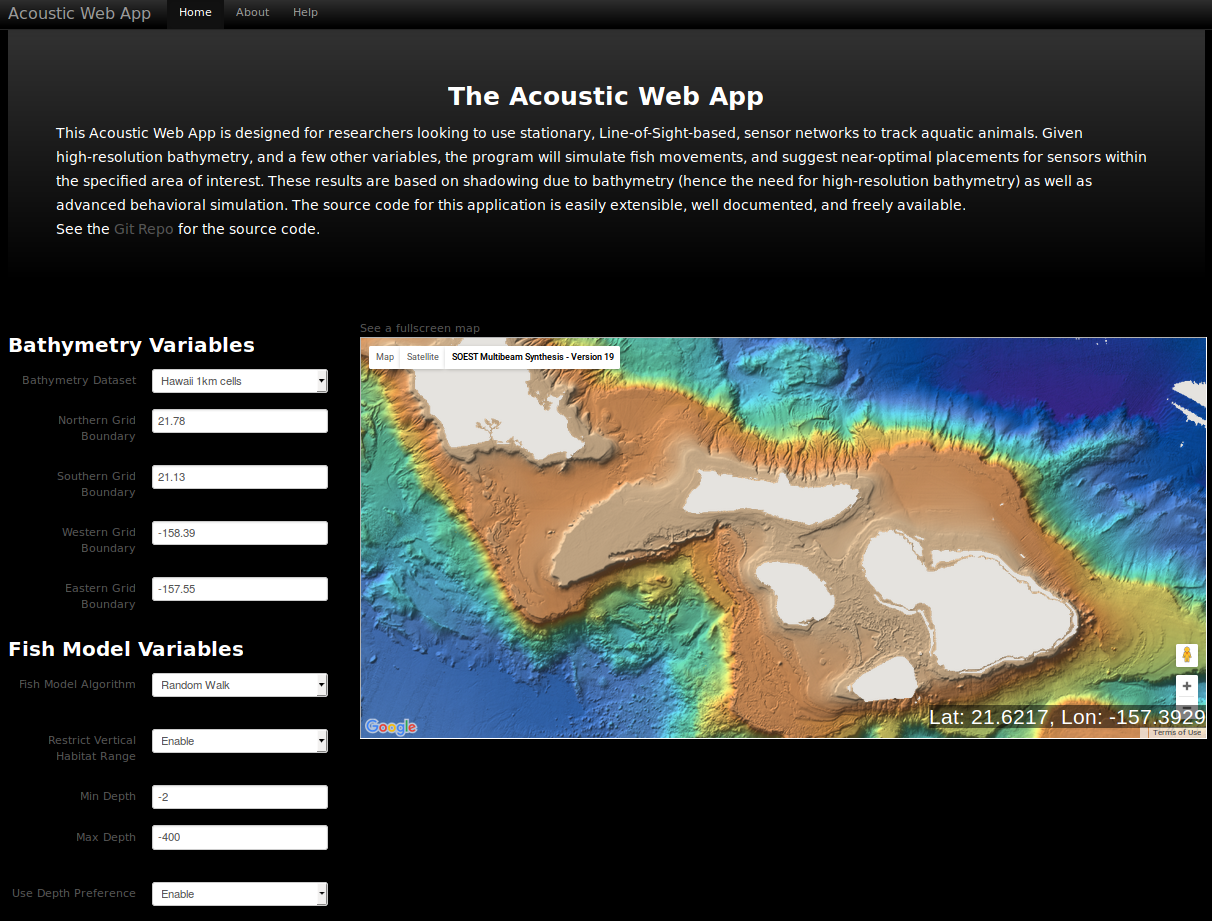
\includegraphics[scale=0.4]{webapp.png}
	\caption{A screenshot of the webapp GUI.  On the right is a Google Map widget that assists users in choosing lattitude and longitude boundaries for their study site (defining their Bathymetry Grid).  On the left is a list of simulation options implemented as drop-down lists, and simulation parameters implemetned as text boxes.  At the bottom (hidden) is a ''Sumbit'' button that sends that validates the parameters and sends them to the server.  All parameters fields and lists display ''tool tip'' style descriptions of the parameter that field/list represents.
		\label{webApp}}
\end{figure}

\subsubsection{Web Server}
\label{webServer}
Included alongside the framework is a web-application (webapp) with a Graphical User Interface (GUI) that runs a simple demonstrative (demo) application using the framework.  The \texttt{Rook} R package is used to handle HTTP interactions between the GUI and the R demo application.  The GUI is a simple HTML page that generates a list of parameters (including a unique $timestamp$ identifier) based on user input, creates a JSON (JavaScript Object Notation) string, and sends an HTTP request to the Rook server with that JSON string.  Using the \texttt{rjson} library, the Rook server decodes the JSON string into R data objects, and calls the demo application using the decoded parameters.  The Rook application signals the successful reception and decoding of the JSON string as an HTTP 200 status update.  The GUI then begins waiting for the completion of the simulation (which may take some time) by continuously checking (ignoring failures) for the existence of a text document (named for the unique $timestamp$ identifier) on the server.  When the simulation finishes its execution (either via error or normal completion), it writes its several output files (Section~\ref{outputFiles}), and a text document containing the JSON representation of the outputs (file paths to graphics and a dictionary of results).  All output files are tagged with a unique $timestamp$ identifier.  Once the GUI finds an output file with the correct $timestamp$ signature, it reads the file, parses the results, and displays them within an HTML page.  If the local system supports it, a zip file of all result files is also supplied.  The webapp serves to simplify the selection and specification of parameters to the demo application.  This allows users to quickly and easily understand the utility of the framework and application.


\subsection{Implementation Hurdles}
\subsubsection{Complexity and Usability}
The primary trade-off that occurs with any application is that between simplicity and control.  While a simpler, less-detailed application may lower the effort required, it inevitably reduces the level of control a users has over the application.  A significant number of variables and options may serve to increase control over an application, but also require increased time and effort to understand and use effectively.  Put simply, very specific actions require very detailed instruction, which in turn requires significant effort.  On the other hand, simpler applications may be more easily understood and adopted, but ultimately lack higher levels of control.  To address this trade-off, both a demo application (Section~\ref{webServer}) and framework are provided.  The demo application provides an easy-to-use application that works ''out-of-the-box'' and has a useful subset of features, while the framework provides access to more detailed functionalities for advanced users.

\subsubsection{Coordinate Conversion}
As mentioned in Section~\ref{bathymetricGrid}, bathymetric files are composed of a regular grid of cells.  However, because the Earth is a 3D sphere, translation is necessary to map that 3D sphere to a 2D grid.  This translation introduces potential error into the specification of a study site.  One such source of error occurs when the method of translation is not specified, leading to ambiguity in how grid cells should be read.  Another possible source of error can be attributed to rounding errors in the number of degrees latitude and longitude represented by each cell.  In grids spanning hundreds of thousands of cells, small rounding errors can lead to large positional discrepancies.  To deal with these issues, the framework requires users to specify their study site as grid cell indexes.  This puts the burden of translating latitude and longitude into gird coordinates on the user (who likely knows best how to handle their data).  Additionally, final receiver placements are given in terms of global (relative to the input bathymetric file) and local (relative to the defined study site) indexes.  This facilitates error checking and helps to identify translational errors.  

\subsubsection{Rook}
The $Rook$ package was selected as a webserver because it offered support for cloud-based web hosting on Heroku and Amazon Web Services (AWS).  This feature was desirable as it allowed users to quickly create a working instance of the web application without modification to their local computers.  Unfortunately, the $Rook$ webserver is implemented using a single, blocking thread.  This means that $Rook$ is only able to handle one request at a time, and will wait for a request to complete before accepting any other other requests.  Because the same Rook thread that receives a request must also call the demo application (which takes about 30 seconds to complete), the entire webserver is unresponsive to new requests until the demo application completes its execution.  This unresponsiveness can lead users to feel like the application is ''frozen'' or ''broken''.  To solve this problem, a loading icon (spinning circle) is used to assure users that the webapp is working.  Another issue with the $Rook$ package is that it imposes a 250 character limit on the length of POST requst data.  Because of the substantial number of parameters sent to the demo application, POST data strings are often very long ($\ge$500 characters).  To compensate, POST data (the JSON string representing user-specified parameters) from the HTML page must to be cut into shorter segments and sent with sequential identifiers and re-assembled on the server.

